\section{Theoretische Grundlagen}
\label{sec:theoretische_grundlagen}

Normalerweise sind Elektronen durch den Potentialverlauf an ihren Festkörper gebunden.
Wird jedoch eine Spannung angelegt und ein Leiter hinreichend nah an diesen herangeführt, kann ein Tunnelstrom erzeugt werden.
Durch schrittweises abtasten der Probe, kann so ein Höhenprofil vermessen werden.
Dies hat den Vorteil, dass die Messung im Realraum stattfindet und auch bei nicht-periodischen Proben angewendet werden kann.
\begin{figure}[!h]
    \centering
    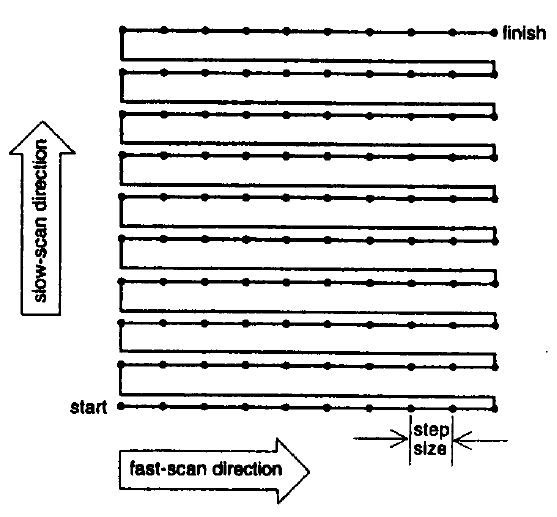
\includegraphics[width=0.4\textwidth]{images/scanning.jpg}
    \caption{Scanner motion during data aquesition \cite{STM-Literatur}}
\end{figure}

\subsection{Tunnelstrom eines Rastertunnelmikroskops} % (fold)
\label{sub:tunnelstrom}

Bei einem Rastertunnelmikroskop wird eine Metallspitze hinreichend nah an den zu untersuchenden Festkörper herangeführt.
Der Tunnelstrom kann nun über die Proportionalität
\begin{equation}
    I_\text{Tunnel} \propto \frac{U}{d} \exp{\left( - K d \sqrt{\Phi} \right)} \label{eqn:tunnelstrom}
\end{equation}
beschrieben werden.
Dabei is $d$ der Abstand zwischen Probe und Leiter, $U$ die angelegte Spannung, $\Phi$ die Austrittsenergie der Probe und $K$ eine Konstante, welche für das Vakuum den Wert $K = \SI{1,025}{\angstrom^{-1} \electronvolt^{-\frac{1}{2}}}$ hat.

\subsection{Rastertunnelmikroskopie} % (fold)
\label{sub:rastertunnelmikroskopie}

Im Folgenden wird näher auf das Rastertunnelmikroskop eingegangen.

\subsubsection{Messmethoden} % (fold)
\label{ssub:messmethoden}

Bei der Rastertunnelmikroskopie wird meist die Methode des konstanten Tunnelstroms gewählt.
Dabei muss der Abstand zwischen Leiterspitze und Probe durchgehend im Bereich von $\SI{0,5}{\angstrom}$ bis $\SI{1,0}{\angstrom}$ gehalten werden, um einen konstanten Tunnelstrom nach Gleichung \ref{eqn:tunnelstrom} zu erhalten.
Die Änderung im Abstand kann nun als elektronisches "`Höhenprofil"' interpretiert werden.

Alternativ wäre es noch möglich, den Abstand zwischen Leiter und Probe konstant zu halten und auf Grund der Änderung des Tunnelstroms Rückschlüsse auf das "`Höhenprofil"' zu ziehen.
Diese Methode ist etwas schneller, doch kann es bei größeren Unregelmäßigkeiten in der Oberfläche zu mechanischem Kontakt zwischen Leiter und Probe kommen, wodurch die Leiterspitze unbrauchbar wäre.

\subsubsection{Voraussetzungen} % (fold)
\label{ssub:voraussetzungen}

Um einen sehr geringen Abstand zwischen Probe und Leiter zu halten und gleichzeitig einen mechanischen Kontakt zu verhindern, muss die Apparatur gut von externen Störquellen abgeschirmt sein.
In diesem Fall befindet sich das Mikroskop auf einem kleinem Tisch, welcher Vibrationen ausgleicht.
Größere Temperaturschwankungen können zu thermischer Drift führen, weshalb sich diesess Experiment an einem schattigen Platz befindet.
Ist eine größere Genauigkeit der Messung vonnöten, sollte das Mikroskop zudem in einer temparierten Umgebung auch vor akkustischen Einflüssen geschützt werden.

Ist die Probe nicht selbst leitend, muss die Oberfläche durch Aufdampfen eines leitenden Materials leitend gemacht werden oder eine dünne Schicht der Probe auf ein leitendes Material aufgebracht werden.
Sollte die Probe aus einem leicht oxidierbarem Material bestehen, sollte der Versuch im Vakuum durchgeführt werden.

\subsubsection{Piezokristalle} % (fold)
\label{ssub:piezokristalle}

Um die Leiterspitze relativ zur Probe mit hoher Genauigkeit bewegen zu können, werden Piezokristalle verwendet.
Diese Keramiken besitzen die Eigenschaft, sich bei Anlegen einer Spannung auszudehnen oder zusammenzuziehen.
Dies lässt sich durch das Ausrichten von Mikrodipolen im Inneren des Materials erklären.
Werden mehrere Piezokristalle verwendet, lassen sich sehr genaue Bewegungen in allen Raumdimensionen im Bereich von  $\SI{0,05}{\angstrom}$ bis $\SI{0,1}{\angstrom}$ erreichen.

Komplikationen treten dabei in verschiedenen Formen auf.
Zum einen steht die angelegte Spannung nur fast in linearem Zusammenhang mit der resultierenden Bewegung, zum anderen führen Hysterese Effekte zu einer Abweichung in der Bewegung von etwa $\SI{15}{\percent}$ bis $\SI{20}{\percent}$.
Diese Effekte lassen sich dadurch minimieren, dass die Probe immer nur in einer Richtung abgefahren wird.
\begin{figure}[!h]
    \centering
    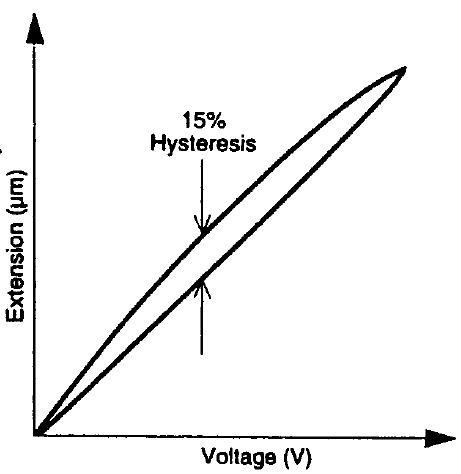
\includegraphics[width=0.4\textwidth]{images/hysterese.JPG}
    \caption{Auswirkung der Hysterese auf die Längenänderung \cite{STM-Literatur}.}
\end{figure}

Ein weiterer Effekt ist das sogenannte Kriechen.
Dies beschreibt die verzögerte Reaktion der Längenänderung auf die Spannungsänderung.
Daher muss bei der Messung nach anlegen der Spannung eine kurze Zeit gewartet werden, bevor die Messung erfolgt.
\begin{figure}[!h]
    \centering
    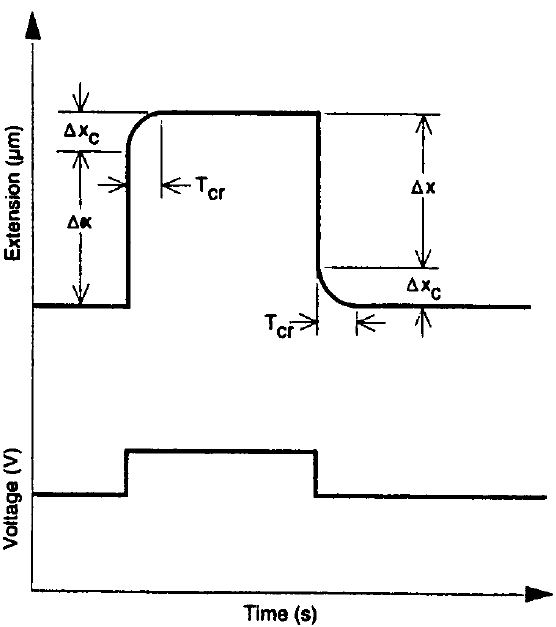
\includegraphics[width=0.4\textwidth]{images/kriechen.JPG}
    \caption{Auswirkungen des Kriechens auf die Längenänderung \cite{STM-Literatur}.}
\end{figure}

Nach einer längeren nicht Benutzung des Kristalls, verliert dieser die Fähigkeit sich bei angelegter Spannung zu verformen, da die Dipole ihre Ausrichtung verlieren.
Durch eine häufige Benutzung kann dieser Effekt wieder Rückgängig gemacht werden.
\begin{figure}[!h]
    \centering
    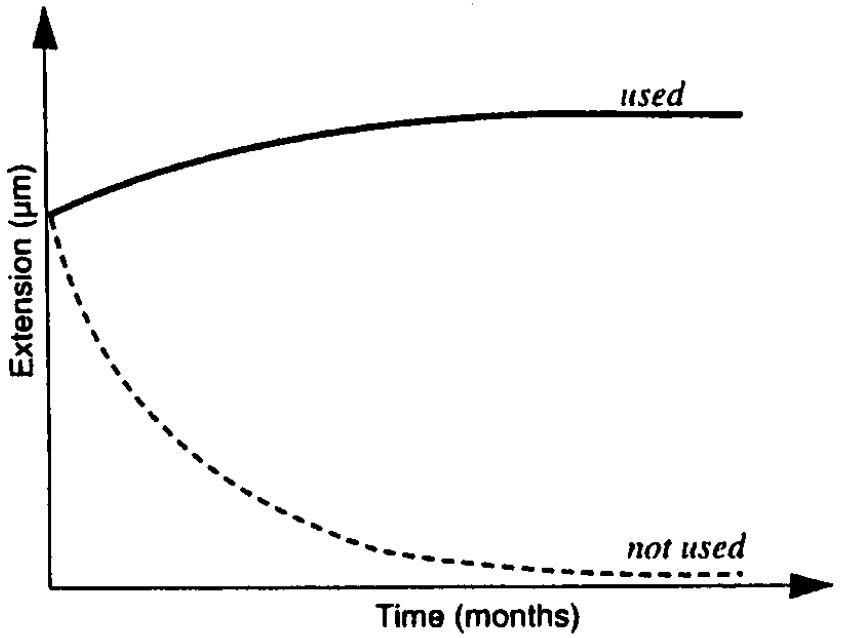
\includegraphics[width=0.4\textwidth]{images/aging.JPG}
    \caption{Auswirkung der Benutzung und nicht Benutzung auf den Piezokristall \cite{STM-Literatur}.}
\end{figure}

Weiterhin kommt es zu einer Kreuzkopplung zwischen x-Achse, y-Achse und der z-Achse.
So kommt es bei einer Änderung der x und y Komponeten auch zu einer Änderung der z Komponente.
Dies führt zu einer Bewegung entlang eines elliptischen Paraboloiden anstatt einer planaren Bewegung.
\begin{figure}[!h]
    \centering
    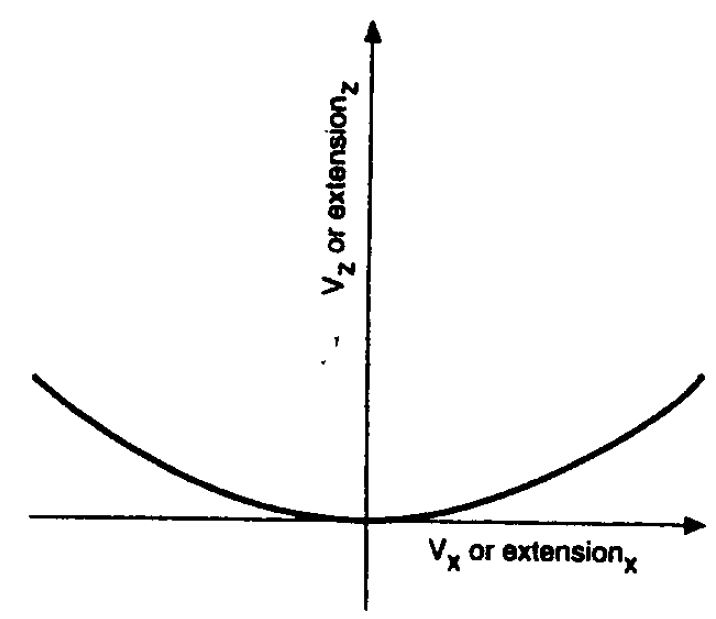
\includegraphics[width=0.4\textwidth]{images/Kreuzkupplung.JPG}
    \caption{Auswirkung der Kreuzkupplung auf die Bewegung der Leiterspitze \cite{STM-Literatur}.}
\end{figure}

Diese Nachteile lassen sich mithilfe einer genauen Kalibrierung und einer Softwarekorrektur nahezu ausgleichen.

\subsection{Untersuchte Proben} % (fold)
\label{sub:proben}

Bei diesem Experiment wird ein synthetisch hergestellter HOPG-Kristall ("`highly ordered pyrolytic graphite"') und Gold verwendet.

\subsubsection{HOPG} % (fold)
\label{ssub:hopg}

HOPG ist eine sehr reine und hoch geordnete Form des Graphits.
Graphit ist eine Reinform des Kohlenstoffs und in zweidimensionalen Schichten angeordnet, welche durch Van-der-Waals Kräfte zusammengehalten werden.
Wie in Abbildung \ref{fig:hopg} dargestellt, bestehen die Schichten aus sechseckig zueinander angeordneten Kohlenstoffatomen (Bienenwaben-Muster), wobei diese um die Hälfte des Abstands $\SI{2,46}{\angstrom}$ zwischen zwei Atomen einer Schicht verschoben sind.
Somit ist die Packungsdichte und die Ordnung des Kristalls sehr hoch und eignet sich somit hervorragend für die Kalibrierung eines Rastertunnelelektronenmikroskops.
\begin{figure}[!h]
    \centering
    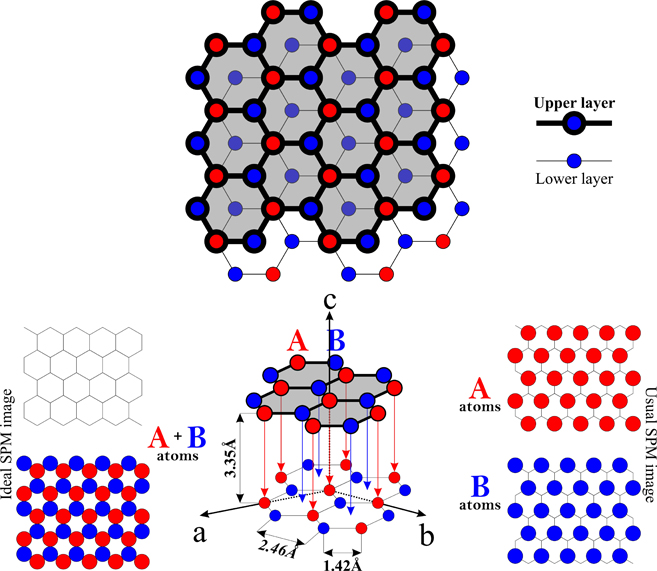
\includegraphics[width=0.4\textwidth]{images/hopg.jpg}
    \caption{Anordnung von HOPG \cite{STM-hopg}.}
    \label{fig:hopg}
\end{figure}

\subsubsection{Gold} % (fold)
\label{ssub:gold}

Gold bildet kubisch flächenzentrierte Kristalle \cite{STM-gold}.
Da die Oberfläche häufig Unebenheiten aufweist, ist diese besonders gut geeignet um das Prinzip der Rastertunnelmikroskopie zu untersuchen.
